\section{有限输入上的可区分模式}
\label{sec:comb-label-family-capacity}

前面用假设空间规定候选预测规则。用观测数据挑选规则时，
我们只看得到每条规则在有限个观测输入上的输出；两条规则若在这些输入上输出相同，数据就无法区分它们。
函数类可以包含无限多个函数，但观察有限个输入时，二值或有限标签输出只有有限种记录，可以用有限集合的计数方法分析；实值输出则先按阈值比较，再计数高低记录。
本节把这些记录称为输出模式，研究两个问题：在给定个数的输入上最多能实现多少种模式；
以及最多能在多少个输入上任意指定输出。前者衡量函数类在有限数据上的区分能力，后者把这种能力概括为非负整数或无穷。
二值输出先给出限制类、生长函数和VC维；多分类输出的标签多于两个，改变一个输出有多种选择，需要区分替代标签的要求；
实值输出则先与固定阈值比较，再考虑离阈值的间隔。

\subsection{二值函数类}
\label{sec:comb-vc-growth}

固定非空输入空间$\mathcal X$与非空函数类$\mathcal H\subseteq\{0,1\}^{\mathcal X}$，
这里$\{0,1\}^{\mathcal X}$表示全部$\mathcal X\to\{0,1\}$函数组成的集合。
每个函数在输入处只输出$0$或$1$，例如判断一封邮件是否为垃圾邮件。以下先固定输入，再比较不同输入上的模式数量。

\subsubsection{生长函数}
\label{sec:comb-binary-restrictions}

\paragraph{限制类}

先把观察范围限制在一组固定输入上，只保留函数在这些位置的输出。这样，即使原函数类无限大，当前可以区分的输出记录仍可能只有有限种。

\begin{definition}[限制类]
设$C=\{x_1,\ldots,x_m\}$为互异输入组成的有限集，并固定所列次序。
把每个函数在这些输入上的取值组成一个向量，所有这样的向量构成限制类（restriction）：
\[
 \mathcal H|_C=\{(h(x_1),\ldots,h(x_m)):h\in\mathcal H\}.
\]
\end{definition}
一个向量是一个可实现的输出模式。不同函数若在$C$上取值相同，只在限制类中计一次。
限制类是$\{0,1\}^m$的子集，所以由乘法规则至多有$2^m$个模式，无论$\mathcal H$本身有多大。
例如取$\mathcal X=\mathbb R$，令$\mathcal H=\{h_a:a\in\mathbb R\}$，
其中阈值函数$h_a(x)=\mathbb I\{x\geq a\}$把阈值右侧标为$1$，左侧标为$0$；
这里$\mathbb I\{\text{条件}\}$在条件成立时取$1$，否则取$0$。
在输入$1,2,3$上，模式只取决于阈值$a$落在哪一段：$a\leq1$时为$111$，$1<a\leq2$时为$011$，
$2<a\leq3$时为$001$，$a>3$时为$000$。所以其限制类只有这四个模式，$8$种零一记录中有一半无法实现。
$a=1.5$与$a=1.8$都产生$011$，但在输入$1.7$上取值不同，所以当前模式相同不等于函数相同。

\paragraph{生长函数}

限制类的大小取决于输入位置。固定输入个数后，对所有输入组取最大的模式数，得到生长函数。
\begin{definition}[生长函数]
  \label{def:growth-function}
  生长函数（growth function）记录$m$个输入上最多能区分多少模式。
  对整数\(m\geq0\)，定义
  \begin{equation}
    \Pi_{\mathcal H}(m)
    =\max_{x_1,\ldots,x_m\in\mathcal X}
    |\{(h(x_1),\ldots,h(x_m)):h\in\mathcal H\}|.
    \label{eq:growth-function}
  \end{equation}
  \(m=0\)时只有一个空标记，故\(\Pi_{\mathcal H}(0)=1\)。
\end{definition}

这里允许输入重复，因此有限输入空间也能讨论任意$m$；重复位置必须取得相同标签。
模式数是$1$到$2^m$之间的整数（函数类非空，所以至少有一个模式），有限个整数中总有最大者，
即使输入组有无限多种，可能取到的模式数也只有这些整数，所以定义中的最大值存在。
对阈值函数类，把$m$个互异点从小到大排为$x_1<\cdots<x_m$，模式由阈值落在
$(-\infty,x_1],(x_1,x_2],\ldots,(x_{m-1},x_m],(x_m,\infty)$中哪一段决定，
共$m+1$段，每段给出不同的模式；输入有重复时互异点更少，模式也更少。故$\Pi_{\mathcal H}(m)=m+1$。
例如$m=3$时，恰是前面的四种模式。

\paragraph{指示函数}

二值函数与子集一一对应：函数$h$确定了取值为$1$的输入组成的集合$h^{-1}(\{1\})$，
反过来，给定$S\subseteq\mathcal X$，函数$\mathbb I_S(x)=\mathbb I\{x\in S\}$称为$S$的\term{指示函数}（indicator function）：
它在$S$上取$1$，在$S$外取$0$。因此限制类中的模式也可以看作$C$的子集，即标为$1$的输入组成的集合，
生长函数就可以用有限子集计数求出。
设$\mathcal X$为无限集，固定整数$k\geq0$，令
\[
 \mathcal H_k=\{\mathbb I_S:S\subseteq\mathcal X,\ |S|\leq k\}.
\]
在$m$个互异输入上，正标签位置可以是任意大小不超过$k$的子集，因此
\[
 \Pi_{\mathcal H_k}(m)=\sum_{j=0}^{\min\{k,m\}}\binom mj.
\]
例如$k=1,m=3$时只有$000,100,010,001$，数量为$1+3=4$。
这里统计的是模式数，没有给这些模式规定概率。

\subsubsection{VC维}
\label{sec:comb-binary-shattering-counts}

\paragraph{打散}

若一组输入的全部二值模式都能实现，就可以在这些输入上任意指定标签。
\begin{definition}[打散]
  \label{def:shattering}
  若对有限互异输入集\(C\)的每个二值标记\((b_1,\ldots,b_m)\)，都存在\(h\in\mathcal H\)满足\(h(x_i)=b_i\)对全部\(i\)成立，就称\(\mathcal H\)\term{打散}（shatter）\(C\)。等价地，\(\mathcal H|_C=\{0,1\}^m\)。
\end{definition}

例如阈值函数能在一个点上实现$0$和$1$，所以能打散单点集。
在$x_1<x_2$上却不能实现$10$：若$x_1\geq a$，必有$x_2\geq a$。
因此任意两个点都不能被阈值函数类打散。

\paragraph{VC维}

VC维把能够被打散的输入集大小概括为一个数。
\begin{definition}[VC维]
  \label{def:vc-dimension}
  \(\mathcal H\)的\term{VC维}（Vapnik--Chervonenkis dimension）为
  \[
    \operatorname{VC}(\mathcal H)
    =\sup\{|C|:C\subseteq\mathcal X,\ |C|<\infty,\ C\text{被}\mathcal H\text{打散}\}.
  \]
  空集总能被非空函数类打散，所以维度可为\(0\)；若任意大有限集都能被打散，则取值为\(+\infty\)。
\end{definition}

由刚才的单点与两点判断，阈值函数类的VC维为$1$。
这个数记录可被任意标记的输入数，不是参数个数：
$h_{a,b}(x)=\mathbb I\{x\geq a+b\}$虽写成两个参数，仍是同一个阈值函数类，VC维仍为$1$。

\paragraph{区间指示函数}

此例取$\mathcal X=\mathbb R$、$\mathcal H=\{h_{a,b}:a,b\in\mathbb R,\ a\leq b\}$，
其中$h_{a,b}(x)=\mathbb I\{a\leq x\leq b\}$。
对$x_1<\cdots<x_m$，非空正标签位置只能是连续块$\{i,i+1,\ldots,j\}$。
每个连续块都可由区间选出，再加上全零模式，得到
\[
 \Pi_{\mathcal H}(m)=1+\sum_{i=1}^m(m-i+1)=1+\frac{m(m+1)}2.
\]
两个点的四种模式均可实现；三个点却不能实现$101$，因为包含两端的区间也包含中点。
所以区间函数类的VC维为$2$。图~\ref{fig:comb-interval-shattering-patterns}显示这两项判断。
\begin{figure}[htbp]
  \centering
  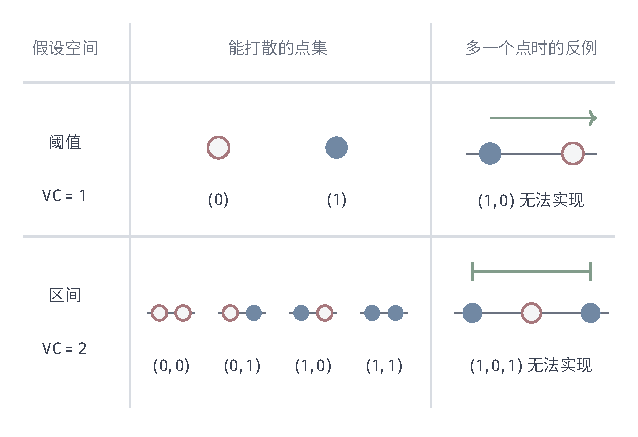
\includegraphics[width=107.999mm]{figures/03-foundations/02-learning-theory/tikz/comb-interval-shattering-patterns/figure.pdf}
  \caption{阈值与单区间函数类的VC维。中列给出能够打散的输入和相应模式；
 右列给出多一个输入时无法实现的模式。实心点表示标签$1$，空心点表示标签$0$；
 箭头表示阈值的正标签向右延续，线段表示包含两个端点的区间也包含中间点。}
 \label{fig:comb-interval-shattering-patterns}
 \label{fig:learning-vc-shattering}
 \label{fig:learning-vc-dimension-examples}
\end{figure}

图~\ref{fig:combinatorics-growth-patterns}比较区间类的模式数与全部$2^m$个二值模式。
计数相同不要求模式相同：$\mathcal H_2$也有$1+m(m+1)/2$个模式，
但在三个点上缺少$111$，区间类缺少的是$101$。
\begin{figure}[htbp]
  \centering
  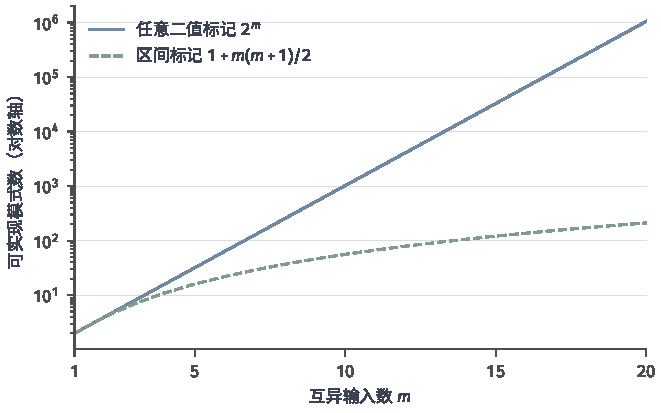
\includegraphics[width=112.0mm]{figures/03-foundations/02-learning-theory/matplotlib/combinatorics-growth-patterns/figure.pdf}
  \caption{有限输入上的二值模式数（精确计数教学图）。蓝实线为不受限制的\(2^m\)，绿虚线为实数轴区间分类器的\(1+m(m+1)/2\)。纵轴使用对数刻度，绿线是该具体类的精确计数；它也恰等于至多两个正类点的集合族计数，但两类实现的模式可以不同。}
  \label{fig:combinatorics-growth-patterns}
  \label{fig:learning-sauer-growth}
\end{figure}

\FloatBarrier
\Needspace{16\baselineskip}
\paragraph{Sauer--Shelah引理}

阈值类和区间类的模式数都只随$m$多项式增长，远小于$2^m$；它们的VC维也都有限。
这不是巧合：只要VC维有限，生长函数就被一个关于$m$的多项式控制。
为了证明这一点，我们把问题从函数类移到有限的模式族上。
固定输入$x_1,\ldots,x_m$后，限制类是一个模式族$\mathcal A\subseteq\{0,1\}^m$。
称$\mathcal A$打散坐标集$I\subseteq\{1,\ldots,m\}$，是指$\mathcal A$中的模式在$I$的坐标上能实现全部$2^{|I|}$种取值；
$\mathcal H$打散输入$\{x_i:i\in I\}$，恰好意味着限制类打散坐标集$I$。
下面的界由删除最后一个坐标后的分类得到。
\begin{lemma}[Sauer--Shelah引理]
  \label{lem:sauer-shelah}
  若\(d=\operatorname{VC}(\mathcal H)<\infty\)，则对任意\(m\geq0\)，
  \[
    \Pi_{\mathcal H}(m)\leq\sum_{j=0}^{\min\{d,m\}}\binom mj.
  \]
  特别地，当\(1\leq d\leq m\)时，
  \begin{equation}
    \Pi_{\mathcal H}(m)\leq\sum_{j=0}^{d}\binom mj
    \leq\left(\frac{em}{d}\right)^d.
    \label{eq:sauer-shelah}
  \end{equation}
\end{lemma}

\begin{proof}
记$\Phi(m,d)=\sum_{j=0}^{\min\{d,m\}}\binom mj$。我们证明更一般的命题：
任何不能打散超过$d$个坐标的模式族$\mathcal A\subseteq\{0,1\}^m$都满足$|\mathcal A|\leq\Phi(m,d)$。
对$\mathcal H$的任一输入组，限制类不能打散超过$d$个坐标（否则相应输入被$\mathcal H$打散，与VC维为$d$矛盾），
所以这个命题给出引理的第一项结论。

先处理边界情形。$m=0$时只有空模式，$|\mathcal A|\leq1=\Phi(0,d)$。
$d=0$时$\mathcal A$不能打散任何单个坐标；若$\mathcal A$含有两个不同模式，它们在某一坐标上分别取$0$和$1$，
就打散了这个坐标，所以$|\mathcal A|\leq1=\Phi(m,0)$。

对$m,d\geq1$，假定命题对$m-1$个坐标、任意维数上界都成立。
把每个模式删去末坐标，所得前缀组成$U\subseteq\{0,1\}^{m-1}$；
令$W\subseteq U$为既能接$0$又能接$1$的前缀，即$u0$与$u1$都属于$\mathcal A$的前缀$u$。
按前缀给$\mathcal A$的模式分类：每个前缀$u\in U$对应一个或两个模式，恰在$u\in W$时对应两个。
加法规则给出$|\mathcal A|=|U|+|W|$。

$U$不能打散超过$d$个坐标：若$U$打散坐标集$I$，则$\mathcal A$中的模式在$I$上也实现全部取值，故$|I|\leq d$。
$W$不能打散$d$个坐标：若$W$打散某个$|I|=d$的坐标集，则对$I$上的任意取值，都有$W$中的前缀实现它，
而该前缀接$0$或接$1$都在$\mathcal A$中，于是$\mathcal A$打散$I\cup\{m\}$这$d+1$个坐标，产生矛盾。
所以$W$不能打散超过$d-1$个坐标。对$U$与$W$分别使用归纳假设，再用Pascal恒等式逐项合并，便得到
\[
  |\mathcal A|
  \leq\sum_{j=0}^{d}\binom{m-1}{j}
       +\sum_{j=0}^{d-1}\binom{m-1}{j}
  =\binom{m-1}0+\sum_{j=1}^{d}\left[\binom{m-1}j+\binom{m-1}{j-1}\right]
  =\sum_{j=0}^{d}\binom mj,
\]
其中超过坐标数的组合数约定为零，因此这也等于$\Phi(m,d)$。重复输入只会减少可独立取值的坐标，不会增大模式数，
因此对全部输入组取最大值得到第一项结论。

简化界另用初等指数不等式$1+u\leq e^u$（$u\geq0$），其中$e$为自然指数的底；
它由指数函数的非负项级数保留前两项得到。
它把有限二项式和写成便于比较的上界，前面的二项式和结论不依赖这一步。
还要比较$\sum_j\binom mja^j$与$(1+a)^m$：把$m$个因子$(1+a)$的乘积逐项展开，
每一项从每个因子中选$1$或$a$；按选出$a$的因子组成的集合分类，选出$j$个$a$的方式恰有$\binom mj$种，每种贡献$a^j$。
因此$\sum_{j=0}^m\binom mja^j=(1+a)^m$，舍去$j>d$的非负项便得下式中的第二个不等号。
当\(1\leq d\leq m\)时，令\(a=d/m\in(0,1]\)。对\(j\leq d\)有\(a^d\leq a^j\)，故
\[
  a^d\sum_{j=0}^{d}\binom mj
  \leq\sum_{j=0}^{d}\binom mj a^j
  \leq(1+a)^m\leq e^{am}=e^d.
\]
除以\(a^d=(d/m)^d\)便得到简化界。\(d=0\)时第一项界为\(1\)，不使用含\(d\)作分母的简化式。
\end{proof}

例如$d=2$时，上界为$1+m+\binom m2$，区间函数类恰好达到它。
这个引理是计数结论；将它用于抽样误差，还需要概率、可测性等条件，
可参考\BookChapterRef{chap:random-sequences-and-processes}{卷2《数学准备：概率、因果与决策》的“随机序列与随机过程”章}。

\subsection{多分类函数类}
\label{sec:comb-multiclass-dimensions}

固定非空输入集合$X$、非空标签集合$Y$和非空函数类$\mathcal H\subseteq Y^X$。
限制类仍记录有限互异输入上的输出向量。二值情形下，打散要求每个输入都能取“另一个”标签，
而另一个标签是唯一的。标签超过两个时，改变一个标签有多种选择，“任意安排输出”就有不同的严格程度：
可以要求在事先固定的两个标签之间任选，可以要求每个模式都能单独改动任一坐标，
也可以只要求能任意决定每个输入是否等于某个参照标签。
下面依次给出这三种要求及相应维数，它们对替代标签的限制由强到弱，最后比较三者的大小关系。

\subsubsection{Natarajan维}
\label{sec:comb-fixed-label-pairs}

\paragraph{Natarajan打散}

Natarajan打散在每个输入上预先固定两个不同标签，再要求实现全部逐点二选一组合。
设$C=\{x_1,\ldots,x_m\}\subseteq X$。若存在$f,g:C\to Y$，
满足每个$x$上$f(x)\neq g(x)$，且对每个$B\subseteq C$都有$h_B\in\mathcal H$满足
\begin{equation}
 h_B(x)=\begin{cases}f(x),&x\in B,\\g(x),&x\in C\setminus B,\end{cases}
 \label{eq:natarajan-shattering}
\end{equation}
就称$C$被$\mathcal H$ \term{Natarajan打散}（Natarajan shattering）。
例如两个输入分别固定标签对$(a,b)$、$(u,v)$时，需要
$(a,u),(a,v),(b,u),(b,v)$四种模式全部出现。

\paragraph{Natarajan维}

固定标签对以后，可以逐个检查哪些输入集允许全部二选一安排。将这些输入集的大小汇总，就得到函数类在这种要求下的维数。

\begin{definition}[Natarajan维]
\label{def:natarajan-dimension}
$\mathcal H$的Natarajan维（Natarajan dimension）为
\[
 d_N(\mathcal H)=\sup\{|C|:C\subseteq X\text{为被}\mathcal H\text{ Natarajan打散的有限集}\}.
\]
没有非空被打散集合时取$0$，可打散任意大有限集时取$+\infty$。
\end{definition}

二标签时，每点的两种标签就是整个$Y$，所以Natarajan维等于VC维。
下面的三标签例子可以逐项检查定义中的四种选择。
\begin{example}[Natarajan维恰为2的有限函数类]
\label{ex:comb-natarajan-concrete}
令输入空间为三封固定邮件$x_1,x_2,x_3$，函数类只含
图~\ref{fig:natarajan-concrete}中的四个函数。在$x_1$上固定标签对“正常、广告”，
在$x_2$上固定“正常、诈骗”，四个函数实现两对标签的全部四种逐点选择，所以
$d_N\geq2$。第三封邮件在四个函数下都预测为正常，任何包含$x_3$的输入集都不能
在该处实现两个不同标签；输入空间只有三点，因此$d_N\leq2$。两项合起来得到
$d_N=2$。
\end{example}

\begin{figure}[htbp]
  \centering
  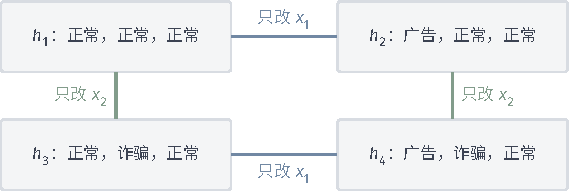
\includegraphics[width=96.28mm]{figures/03-foundations/02-learning-theory/tikz/natarajan-concrete/figure.pdf}
  \caption{Natarajan打散的四种预测。每个框中的三项依次对应$x_1,x_2,x_3$；
 横向只改变$x_1$，纵向只改变$x_2$，而$x_3$始终预测为正常。
 每个输入处的两个标签预先固定，四个函数实现全部二选一组合。}
 \label{fig:natarajan-concrete}
\end{figure}
\FloatBarrier

\paragraph{生长函数}

当$|Y|=K<\infty$时，沿用式~\eqref{eq:growth-function}对所有输入组取最大值，
定义多分类生长函数$\Pi_{\mathcal H}(m)$，它至多为$K^m$。
有限Natarajan维可将这一上界改进为下面的二项式和。
\begin{theorem}[有限标签的预测数目上界]
\label{thm:multiclass-growth-bound}
设\(2\leq |Y|=K<\infty\)，\(d=d_N(\mathcal H)<\infty\)。
记\(q=\binom K2=K(K-1)/2\)为不同无序标签对的数目，则对每个整数\(m\geq0\)，
\begin{equation}
  \Pi_{\mathcal H}(m)\leq G_{d,K}(m)
  :=\sum_{j=0}^{\min\{d,m\}}\binom mj q^j.
  \label{eq:comb-multiclass-growth-bound}
\end{equation}
\end{theorem}

\begin{proof}
将有限非空模式族\(V\subseteq Y^m\)视为坐标集\(\{1,\ldots,m\}\)上的函数类，
并设其Natarajan维至多为\(d\)。删去末坐标得到前缀族\(U\subseteq Y^{m-1}\)。
对\(u\in U\)，记它能够接上的末尾标签数为\(r(u)\geq1\)。按前缀分类，\(|V|=\sum_{u\in U}r(u)\)，
而\(|U|=\sum_{u\in U}1\)，所以\(|V|-|U|=\sum_u(r(u)-1)\)。
对每个不同标签对\(\{a,b\}\)，令\(U_{a,b}\)为既能接上\(a\)又能接上\(b\)的前缀族。
一个前缀属于\(U_{a,b}\)，当且仅当\(\{a,b\}\)是它能接上的\(r(u)\)个标签中的一对，所以它恰属于\(\binom{r(u)}2\)个\(U_{a,b}\)，
即\(\sum_{\{a,b\}}|U_{a,b}|=\sum_u\binom{r(u)}2\)。又因\(r\geq1\)时\(r-1\leq r(r-1)/2=\binom r2\)，对前缀求和可得
\[
  |V|\leq |U|+\sum_{\substack{\{a,b\}\subseteq Y\\a\neq b}}|U_{a,b}|.
\]
每个无序对在求和中只出现一次。\(U\)的Natarajan维至多为\(d\)。当\(d\geq1\)
时，每个非空\(U_{a,b}\)的Natarajan维至多为\(d-1\)：否则它可以在某\(d\)个
坐标上实现全部固定标签对的选择；每个对应前缀又能接上\(a\)或\(b\)，使\(V\)
在这\(d\)个坐标与末坐标上实现全部二元选择，违反维度上界。空\(U_{a,b}\)的
计数贡献为零。

记\(M(m,d)\)为Natarajan维至多\(d\)的非空模式族\(V\subseteq Y^m\)能够达到的
最大大小，标签集\(Y\)保持固定。对\(m,d\geq1\)，上述分组给出
\[
  M(m,d)\leq M(m-1,d)+qM(m-1,d-1).
\]
零个坐标只有一个空模式，故\(M(0,d)=1\)。维度为零时也至多有一个模式：两个
不同模式必在某坐标上取不同标签，从而Natarajan打散一个坐标。因此\(M(m,0)=1\)。
对\(m\)归纳，将两个较小问题的上界代入，并使用二项式递推关系，得到
\[
\begin{aligned}
  M(m,d)
  &\leq\sum_{j=0}^{d}\binom{m-1}{j}q^j
       +q\sum_{j=0}^{d-1}\binom{m-1}{j}q^j\\
  &=\sum_{j=0}^{d}\binom mj q^j,
\end{aligned}
\]
其中超出坐标数的组合数约定为零。任意输入组上的限制类，其Natarajan维不超过
\(d_N(\mathcal H)\)；重复输入不能作为两个可独立选择的坐标。因此对输入组取最大值，
得到式~\eqref{eq:comb-multiclass-growth-bound}。
\end{proof}

例如$K=3,d=1,m=4$时，$q=3$，界为$1+4\times3=13$，小于全部$3^4=81$种模式。
$K=2$时$q=1$，该公式恢复Sauer--Shelah计数界。

\subsubsection{DS维}
\label{sec:comb-coordinate-replacements}

\paragraph{伪立方体}

另一种要求是不固定标签对，而让每个模式都能单独改变任一坐标，并仍留在同一个有限模式族中。
\begin{definition}[伪立方体]
\label{def:pseudocube}
有限非空集合$V\subseteq Y^m$称为$m$维伪立方体，如果对每个$v\in V$和
每个$i\in\{1,\ldots,m\}$，都存在$u\in V$满足
$u_i\neq v_i$且$u_j=v_j$对所有$j\neq i$成立。
\end{definition}

例如取三个互异标签$a,b,c$，
\[
 \mathcal V=\{(a,a),(a,b),(b,b),(b,c),(c,c),(c,a)\}
\]
是二维伪立方体：每个模式沿第一、第二坐标都能找到一个邻居。
它却不含固定两标签对形成的四个角。图~\ref{fig:comb-multiclass-pattern-grid}把六个模式列入表格，
每行每列都有两个模式，但没有完整的二行二列矩形。
\begin{figure}[htbp]
  \centering
  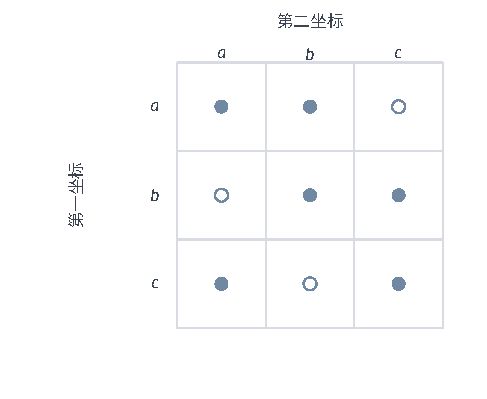
\includegraphics[width=82.501mm]{figures/03-foundations/02-learning-theory/tikz/comb-multiclass-pattern-grid/figure.pdf}
  \caption{六模式族$\mathcal V$的精确占位图。实心点表示模式属于该族，空心点表示缺失模式。每行每列恰有两个实心点，却没有完整的四角矩形；这不是两个标签的完整立方体。}
 \label{fig:comb-multiclass-pattern-grid}
\end{figure}

\paragraph{DS打散}

若$m$个互异输入组成的有序点集$C$满足$\mathcal H|_C$包含一个$m$维伪立方体，
称$C$被\term{DS打散}（DS shattering）。例如把上述六模式作为两个输入上的全部限制类，
这两个输入便被DS打散，因为六个模式构成二维伪立方体。

\paragraph{DS维}

把能够逐坐标替换的输入规模汇总，就得到Daniely--Shalev-Shwartz维，简称DS维；
下面采用有限伪立方体的表述\scite{brukhim2022multiclass}。
\begin{definition}[DS维]
\label{def:ds-dimension}
DS维$d_{DS}(\mathcal H)$为可被DS打散的有限输入集大小的上确界。
空集给出大小$0$；若任意大的有限集都能被DS打散，维数取$+\infty$。
\end{definition}

对只有两个输入的函数类$\mathcal V$，上述六个模式构成二维伪立方体，因此$d_{DS}=2$。
没有四角矩形意味着不能Natarajan打散两个输入，而一个输入可以取不同标签，故$d_N=1$。
图~\ref{fig:ds-six-cycle}标出每个模式沿两个坐标的邻居。
\begin{figure}[htbp]
  \centering
  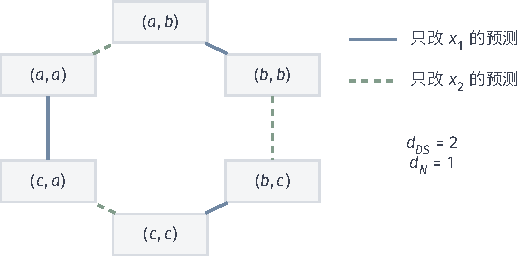
\includegraphics[width=89.02mm]{figures/03-foundations/02-learning-theory/tikz/ds-six-cycle/figure.pdf}
  \caption{六模式族$\mathcal V$的逐坐标邻接。每个顶点是一种两输入预测；
 蓝实线只改变第一坐标，绿虚线只改变第二坐标。每个顶点在两个方向上都有邻居，
 所以它构成二维伪立方体；图中没有固定两标签对形成的四角矩形，故其
 DS维为2而Natarajan维为1。}
 \label{fig:ds-six-cycle}
\end{figure}

\FloatBarrier
\subsubsection{图维}
\label{sec:comb-reference-labels}

\paragraph{图打散}

图打散先固定每点的参照标签，再要求任意一部分输入匹配参照、其余输入不匹配。
不匹配时采用哪个标签不必预先指定。
\begin{definition}[图打散]
\label{def:graph-dimension}
若有限集$C\subseteq X$存在$f:C\to Y$，使每个$B\subseteq C$都对应某个
$h_B\in\mathcal H$，满足
\[
 h_B(x)=f(x)\ (x\in B),\qquad h_B(x)\neq f(x)\ (x\in C\setminus B),
\]
则称$C$被$\mathcal H$图打散。
\end{definition}

例如参照标签为$(a,u)$时，$(a,u),(a,v),(b,u),(c,w)$分别实现全匹配、只匹配第一处、
只匹配第二处和全不匹配，其中$v\neq u$、$b,c\neq a$、$w\neq u$。

\paragraph{图维}

图打散判断一组输入能否独立安排匹配与不匹配。把能够这样安排的输入数概括为一个上界，就得到对应的维数。

\begin{definition}[图维]
\label{def:graph-dimension-value}
图维（graph dimension）记录可独立安排这种匹配关系的最大点数。
设$\mathcal C_G$为所有被$\mathcal H$图打散的有限输入集组成的集合，定义
\[
 d_G(\mathcal H)=\sup_{C\in\mathcal C_G}|C|.
\]
\end{definition}

\begin{example}[图维恰为2的有限函数类]
\label{ex:comb-graph-shattering-concrete}
令输入空间为$\{x_1,x_2,x_3\}$，函数类只含图~\ref{fig:graph-shattering-concrete}
中的四个函数。以$f(x_1)=a,f(x_2)=u$为基准，四个函数在前两个输入上分别实现
“两处都匹配、只匹配第一处、只匹配第二处、两处都不匹配”，所以
$\{x_1,x_2\}$被图打散。第三个输入始终取$z$，任何包含$x_3$的集合都不能在该处
独立安排匹配与不匹配；输入空间又只有三个点，故这个函数类的图维恰为2。
\end{example}

\begin{figure}[htbp]
  \centering
  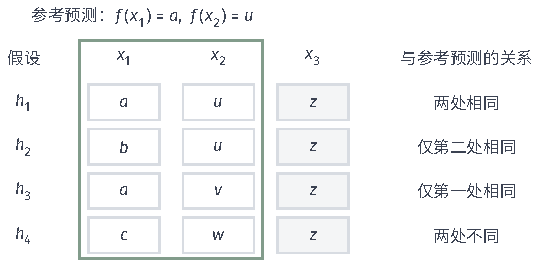
\includegraphics[width=91.401mm]{figures/03-foundations/02-learning-theory/tikz/graph-shattering-concrete/figure.pdf}
  \caption{图打散与图维的有限例子。框线圈定的两列相对于参考函数实现全部四种匹配或
 不匹配组合；第三列固定为$z$。同一输入偏离基准时可以采用不同标签，
 因而图打散没有预先固定唯一的替代标签。}
 \label{fig:graph-shattering-concrete}
\end{figure}

\paragraph{维数比较}

三种维数分别要求固定标签对、逐坐标邻居和匹配参照标签，按对替代标签的限制由强到弱排列。
表~\ref{tab:comb-multiclass-dimensions}列出条件，图~\ref{fig:learning-multiclass-dimensions}显示对应模式。
\begin{table}[htbp]
  \centering
  \begin{tabular}{p{0.17\linewidth}p{0.70\linewidth}}
    \toprule
    维度 & 在有限输入上的要求\\
    \midrule
    Natarajan维 & 每点固定两个不同标签，全部\(2^m\)种逐点二选一组合均可实现\\
    DS维 & 包含有限非空模式族，每个模式在任一坐标都可单独改变并仍留在族中\\
    图维 & 每点固定一个基准标签，任意点集上匹配、其补集上不匹配的模式均可实现\\
    \bottomrule
  \end{tabular}
  \caption{多类别组合维度的不同量词。图维中的“图”指标记相等关系的图打散，不是输入关系图的顶点数。}
  \label{tab:comb-multiclass-dimensions}
\end{table}

\begin{figure}[htbp]
  \centering
  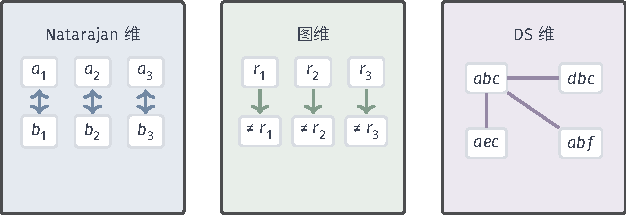
\includegraphics[width=106.056mm]{figures/03-foundations/02-learning-theory/tikz/learning-multiclass-dimensions/figure.pdf}
  \caption{多分类维度关注的三种结构。Natarajan维固定每个输入处的两个标签，
 图维固定一个基准标签并区分匹配与不匹配，DS维考察预测向量之间只改变一个坐标的
 邻接。右栏只展示局部邻接方式；完整伪立方体还要求每个模式在每个坐标上都有邻居。}
 \label{fig:learning-multiclass-dimensions}
\end{figure}
\FloatBarrier

三种打散要求对替代标签作出的限制不同，但同一组预测模式可以同时接受这些检验。下面比较由这些要求得到的维数，并说明标签数有限时还能推出什么。

\begin{theorem}[多分类维度的比较]
\label{thm:multiclass-dimension-comparison}
对任意非空标签空间与非空函数类，有
\[
  d_N(\mathcal H)\leq d_{DS}(\mathcal H)\leq d_G(\mathcal H).
\]
二标签时三者均等于VC维。若\(|Y|=K<\infty\)，则\(d_N(\mathcal H)<\infty\)
也蕴含\(d_G(\mathcal H)<\infty\)。
\end{theorem}

\begin{proof}
若\(m\)个输入被Natarajan打散，每个坐标的两个候选标签固定，全部\(2^m\)种
选择组成一个有限非空模式族。任意模式都能只翻转任一坐标上的选择并仍留在族中，
所以它是\(m\)维伪立方体，证明\(d_N\leq d_{DS}\)。

若限制类包含\(m\)维伪立方体\(V\)，固定\(v\in V\)作为基准。任取希望偏离基准
的坐标集\(I\subseteq\{1,\ldots,m\}\)，逐个沿\(I\)中的坐标移动到邻居，每个
坐标只移动一次。每一步仅改变当前坐标；之前改变的坐标保持不变，\(I\)之外的
坐标始终与\(v\)相同。因此最终模式恰在\(I\)上不等于\(v\)，在其补集上等于
\(v\)。令\(I\)遍历所有子集就得到图打散，故\(d_{DS}\leq d_G\)。

二标签时，偏离基准的标签唯一。图打散因此要求全部二元模式；伪立方体从任意模式
逐坐标翻转也能到达全部二元模式。Natarajan打散中的两标签正是整个标签集，所以
三种维度都等于VC维。

若\(K=1\)，函数类在任何输入上只有一种标记，三种维度均为零。若\(2\leq K<\infty\)
且\(d_N=d<\infty\)，图打散\(m\)个输入至少需要\(2^m\)个不同模式。由定理~
\ref{thm:multiclass-growth-bound}，必有\(2^m\leq G_{d,K}(m)\)。固定\(d,K\)后，
当$d=0$时，右侧为$1$，所以只能有$m=0$。当$d\geq1$且$m\geq2(d+1)$时，
大小为$d+1$的子集只是全部$2^m$个子集中的一类，再利用组合数的连乘公式，可得
\[
 2^m\geq\binom m{d+1}\geq\frac{(m/2)^{d+1}}{(d+1)!},
 \qquad
 G_{d,K}(m)\leq C m^d,
\]
其中$C=\sum_{j=0}^d q^j/j!$只依赖$d,K$。与$2^m\leq G_{d,K}(m)$合并并约去$m^d$，
得到$m\leq2^{d+1}(d+1)!C$。较小的$m<2(d+1)$也已有有限上界，故图维有限。
\end{proof}

六模式族$\mathcal V$以$(a,a)$为参照时，$(a,a),(a,b),(c,a),(b,b)$实现四种匹配安排，
所以$d_G=2$。该例的三个维数依次为$1,2,2$。
有限标签条件用于计数界。例如无限标签集$Y$上的全部常值函数$h_y(x)=y$，
三个维数都为$1$，但在单个输入上已有无限多个模式，不能套用含有限$K$的计数公式。

\subsection{实值函数类}
\label{sec:comb-real-valued-threshold-margins}

以下固定非空输入空间$\mathcal X$与非空函数类$\mathcal F\subseteq\mathbb R^{\mathcal X}$。
实数输出在单点上就可能无限多；与其计数精确数值，可以先固定每个输入的阈值，
只记录输出在阈值哪一侧。加入正间隔后，还能描述在给定尺度下能否作出这些选择。

\subsubsection{伪维}
\label{sec:comb-threshold-patterns}

\paragraph{伪打散}

实值函数在单个输入上就能取无限多个值，若按精确数值计数，限制类往往无限，前面的计数没有意义。
把实数输出转化为二值信息的最直接办法，是与一个阈值比较，只记录输出在阈值上方还是下方。
对每个输入先选一个阈值，再检查全部高低组合是否可由函数实现，这称为伪打散。
阈值对全部模式保持不变，实现不同模式的函数则可以不同。
\begin{definition}[伪打散]
\label{def:pseudo-shattering}
设$\mathcal F\subseteq\mathbb R^{\mathcal X}$。有限集$C=\{x_1,\ldots,x_m\}$被
$\mathcal F$\term{伪打散}（pseudo-shattering），是指存在$r_1,\ldots,r_m\in\mathbb R$，使任意
$\bm b\in\{0,1\}^m$都对应某个$f_{\bm b}\in\mathcal F$，满足
\[
 b_i=1\Rightarrow f_{\bm b}(x_i)>r_i,\qquad
 b_i=0\Rightarrow f_{\bm b}(x_i)<r_i\quad(1\leq i\leq m).
\]
这里$\Rightarrow$表示“只要左侧条件成立，右侧便须成立”。
\end{definition}

例如取常值函数类$\mathcal F=\{f_a:a\in\mathbb R\}$，其中$f_a(x)=a$。
在一个输入处取阈值$0$，用$a=1$和$a=-1$便能实现高、低两种模式。
两个输入则不能被它伪打散：若阈值$r_1\leq r_2$，要求第一处低于$r_1$、第二处高于$r_2$，
同一个常数不可能同时满足；$r_2\leq r_1$时交换两处即可。

\paragraph{伪维}

常值函数的例子表明，可任意安排高低模式的输入数可能受到限制。伪维用一个数记录这种独立选择能够覆盖的输入规模。

\begin{definition}[伪维]
\label{def:pseudo-dimension}
$\mathcal F$的\term{伪维}（pseudo-dimension）为
$\operatorname{Pdim}(\mathcal F)=\sup\{|C|:C\text{为被}\mathcal F\text{伪打散的有限集}\}$，
允许值为$+\infty$；没有非空被打散集合时值为$0$。
\end{definition}

由刚才的一点、两点判断，常值实函数类的伪维为$1$。
对二值函数类取阈值$1/2$，伪打散就是VC打散，因此伪维与VC维一致。

\subsubsection{胖打散维}
\label{sec:comb-margin-patterns}

\paragraph{胖打散}

\term{胖打散}（fat shattering）要求输出不仅位于阈值两侧，还要与阈值相距至少一个给定正数$\gamma$。
\begin{definition}[胖打散]
\label{def:fat-shattering}
给定$\gamma>0$，若有限集$C=\{x_1,\ldots,x_m\}$存在固定阈值$r_1,\ldots,r_m$，
使任意$\bm b\in\{0,1\}^m$均对应$f_{\bm b}\in\mathcal F$满足
\begin{equation}
 b_i=1\Rightarrow f_{\bm b}(x_i)\geq r_i+\gamma,\qquad
 b_i=0\Rightarrow f_{\bm b}(x_i)\leq r_i-\gamma,
 \label{eq:fat-shattering}
\end{equation}
则称$C$在尺度$\gamma$下被$\mathcal F$胖打散。
等价地，以$\sigma_i=2b_i-1$编码，可写为
\begin{equation}
 \sigma_i\bigl(f_{\bm\sigma}(x_i)-r_i\bigr)\geq\gamma
 \quad(i=1,\ldots,m).
 \label{eq:functional-fat-shattering}
\end{equation}
\end{definition}

例如输入空间只有一个点，函数类在该点的输出只能取$19.999$和$20.001$，固定阈值$20$。
它能实现高、低两种模式，并能留下间隔$\gamma=0.001$，却不能留下间隔$1$。
这说明跨过阈值和以给定幅度跨过阈值是不同要求。

\paragraph{胖打散维}

同一函数类在不同间隔要求下，能够独立安排的输入数可能不同。固定尺度后，再汇总所有满足胖打散要求的输入集大小，就得到相应的维数。

\begin{definition}[胖打散维]
\label{def:fat-shattering-dimension}
尺度$\gamma$下的\term{胖打散维}（fat-shattering dimension）为
$\operatorname{fat}_\gamma(\mathcal F)=
\sup\{|C|:C\text{为在尺度}\gamma\text{下被}\mathcal F\text{胖打散的有限集}\}$。
采用与伪维相同的$0$及$+\infty$约定。
\end{definition}

固定尺度后，胖打散维记录能同时满足该间隔要求的输入数目。
例如上面只有两个常值输出的函数类，在$0<\gamma\leq0.001$时维数为$1$，在$\gamma>0.001$时为$0$。

\paragraph{单调性}

增大$\gamma$只会加强要求，所以$\operatorname{fat}_\gamma(\mathcal F)$关于$\gamma$单调不增。
因$\gamma>0$保证每个见证严格位于阈值一侧，还得到
$\operatorname{fat}_\gamma(\mathcal F)\leq\operatorname{Pdim}(\mathcal F)$。
反过来，一个被伪打散的固定有限集，在某个正尺度下也被胖打散：
从有限种模式各选一个见证函数，取它们在各输入处距阈值的最小距离即可。
这个距离为正，但依赖输入集和所选函数，不能替代预先指定的尺度。

\Needspace{8\baselineskip}
\paragraph{分块常值函数}

下面用可以直接计算的函数类说明幅度限制的作用。
\begin{example}[分块常值函数的胖打散维]
\label{ex:comb-piecewise-constant-fat-dimension}
设非空集合$A_1,\ldots,A_m$构成$\mathcal{X}$的一个划分，并令
\[
  \mathcal{F}_B
  =
  \left\{
    \sum_{j=1}^{m}a_j\mathbb{I}_{A_j}:
    |a_j|\leq B
  \right\},
  \qquad B>0.
\]
当$0<\gamma\leq B$时，从每个$A_j$选一点并取阈值$r_j=0$；对任意符号模式令
$a_j=\gamma\sigma_j$，便能以间隔$\gamma$实现该模式，所以这$m$个点被胖打散。反过来，
任意$m+1$个点中至少两个落在同一个$A_j$内，而类中每个函数在这两个点取值相同。若二者
的阈值为$r$与$r'$且能够被胖打散，模式$(+1,-1)$要求$r'-r\geq2\gamma$，模式
$(-1,+1)$又要求$r-r'\geq2\gamma$，二者矛盾。因此该尺度下的胖打散维恰为$m$。
当$\gamma>B$时，
单点上的两个符号也要求函数值之差至少为$2\gamma$，超过允许区间$[-B,B]$的宽度$2B$，
故胖打散维为$0$。这个算例把分区数控制的自由方向与系数上界控制的可分辨幅度分开了。
\end{example}

图~\ref{fig:comb-fat-margin-output-square}取两个分块、$B=1$，
把两处输出表示为平面中的一个点。四种高低模式能否实现，取决于间隔区域是否仍与允许的正方形相交。
\begin{figure*}[htbp]
  \centering
  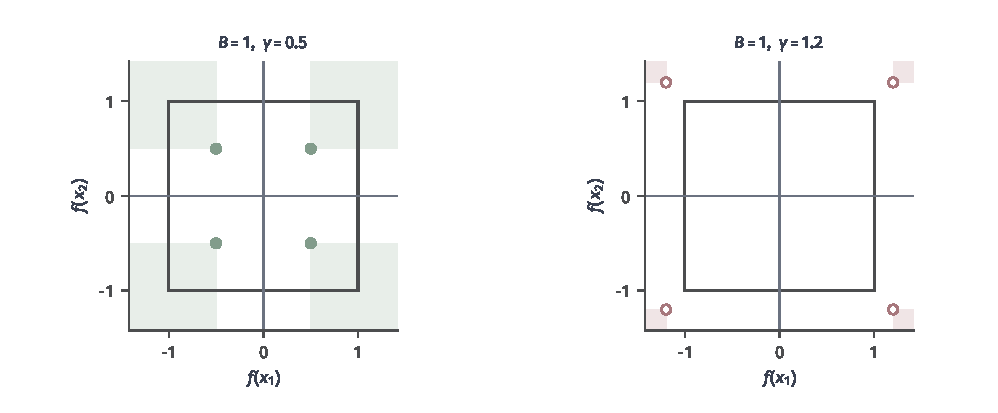
\includegraphics[width=169.0mm]{figures/03-foundations/02-learning-theory/matplotlib/comb-fat-margin-output-square/figure.pdf}
  \caption{两个分块、$B=1$与固定阈值$r_1=r_2=0$的输出几何。灰框是函数类允许的
 $(f(x_1),f(x_2))\in[-1,1]^2$；浅色区域要求两坐标分别离阈值至少$\gamma$。
 左图的浅绿区域对应$\gamma=0.5$，四种符号可由实心点实现；右图的浅红区域对应$\gamma=1.2$，空心点只标出要求的边界，
 全部落在允许框之外，因而不是类中的函数输出。图为解析教学构造。}
 \label{fig:comb-fat-margin-output-square}
 \label{fig:fat-shattering-example}
\end{figure*}

限制类记录具体模式，生长函数记录模式数，打散维数记录满足相应打散条件的输入规模。
实值函数的伪维与胖打散维分别采用固定阈值和正间隔。
它们与函数空间中的距离、覆盖数是不同概念；覆盖数需要先指定比较函数的距离与误差精度，用一组代表近似整个函数类，不能由模式数直接替代；相关空间观点可参考\BookChapterRef{chap:functional-analysis-and-approximation}{卷1《数学准备：计算、分析与几何》的“函数空间”章}。

